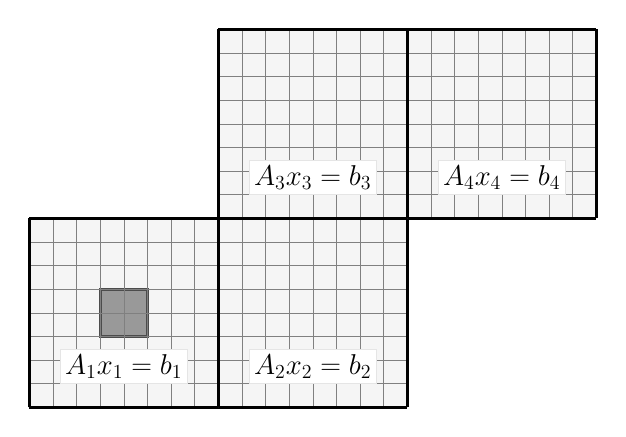
\begin{tikzpicture}
[
scale=0.6,
every node/.style ={scale=0.6},
Background/.style={rectangle,draw=black!04,fill=black!04, thin, minimum size = 4 cm},
Obstruction/.style={rectangle,draw=black!70,fill=black!40, very thick, minimum size=1cm},
Finegrid/.style={step=0.5cm,gray,very thin},
Thickline/.style={-,draw=black!100,fill=black!02, very thick},
Thinline/.style={draw=black!100,fill=black!02, very thin},
Ball/.style={circle, draw=black!40, fill=red!20, thin, minimum size=3.5mm},
Circle/.style={circle,draw=black!40,fill=black!06,thin,minimum size=35.5mm},
%Rectangle/.style={rectangle,color=blue, inner xsep=7pt, inner ysep=7pt,},
%Rectangle/.style={rectangle,color={rgb,255:red,192;green,58;blue,10}, inner xsep=7pt, inner ysep=7pt,},
Rectangle/.style={rectangle,draw=black!10,fill=white,inner xsep=3pt, inner ysep=3pt,},
box/.style = {very thin, rectangle, inner xsep=10pt, inner ysep=10pt,},
]

\node[Background] at (2,2) {};
\node[Background] at (6,2) {};
\node[Background] at (6,6) {};
\node[Background] at (10,6) {};

\node[Obstruction] at (2,2) {};

\draw[Finegrid] (0,0) grid (8,4);
\draw[Finegrid] (4,4) grid (12,8);

\draw[Thickline] (0,0)--(8,0);
\draw[Thickline] (4,8)--(12,8);
\draw[Thickline] (0,4)--(4,4);
\draw[Thickline] (8,4)--(12,4);

\draw[Thickline] (0,0)--(0,4);
\draw[Thickline] (4,8)--(12,8);
\draw[Thickline] (4,4)--(4,8);
\draw[Thickline] (8,0)--(8,4);
\draw[Thickline] (12,4)--(12,8);

\draw[Thickline] (4,0)--(4,4);
\draw[Thickline] (4,4)--(8,4);
\draw[Thickline] (8,4)--(8,8);

\node[Rectangle] at ( 2,0.86) {\LARGE $\boldsymbol{A_1x_1=b_1}$};
\node[Rectangle] at ( 6,0.86) {\LARGE $\boldsymbol{A_2x_2=b_2}$};
\node[Rectangle] at ( 6,4.86) {\LARGE $\boldsymbol{A_3x_3=b_3}$};
\node[Rectangle] at (10,4.86) {\LARGE $\boldsymbol{A_4x_4=b_4}$ };

\vspace{4cm}

%\node[Rectangle] at (16,2) {\textcolor{hhpred} {\Huge $ x \,\overset{ \mbox{\raisebox{1mm}{?}}}{=}\, \summv x_i$}};

\end{tikzpicture}
